% Copyright 2007 by Till Tantau
% Copyright 2014 by Rich Wareham, Filippo Spiga
% Copyright 2016 by Petar Veličković
% Copyright 2020 by Shivam N Patel
% This file may be distributed and/or modified:
% 1. under the LaTeX Project Public License and/or
% 2. under the GNU Public License.
%
% See the file LICENSE for more details.

\documentclass{beamer}

\usetheme{cambridge} 

\setbeamertemplate{navigation symbols}{}  % suppress navigation symbols
\setbeamertemplate{footline}[text line]{%
  \parbox{\linewidth}{\vspace*{-8pt}Sam Leeney - sakl2@cam.ac.uk \hfill arxiv: 2211.15448 \hfill\insertpagenumber}}
%%% Standard packages:
\usepackage[english]{babel}
\usepackage[latin1]{inputenc}
\usepackage{graphicx}
\usepackage{multicol}
\usepackage{subfigure}
\usepackage{listings}
\usepackage[UKenglish]{isodate}
\usepackage{animate}

% Setup TikZ

\usepackage{tikz}
\usetikzlibrary{arrows}
\tikzstyle{block}=[draw opacity=0.7,line width=1.4cm]

\cleanlookdateon

% Author, Title, etc.

\title[Cross-modal convnets] 

}
\author[Veli\v{c}kovi\'{c} et al.]
{Samuel AK Leeney (sakl2@cam.ac.uk)}
\institute[CL]
{Developed in collaboration with Will Handley and Eloy de Lera Acedo}

\date[ARMRS2016]
{Astrostatistics and Astro-Machine Learning Workshop \hfill \today}
% The main document

\begin{document}

\begin{frame}
  \titlepage
  \begin{tikzpicture}[remember picture, overlay]
    \node[right=4.1cm, above=3.2cm] at (current page.center) 
    {
    
\includegraphics[width=0.3\textwidth]{eddies.png}
    };
    \end{tikzpicture}

  \begin{tikzpicture}[remember picture, overlay]
    \node[right=0cm, above=3cm] at (current page.center) 
    {
    
\includegraphics[width=0.25\textwidth]{output-onlinepngtools.png}
    };
  \end{tikzpicture}
  
\end{frame}

\begin{frame}{What is RFI?}
\begin{columns}
\column{0.5\textwidth}
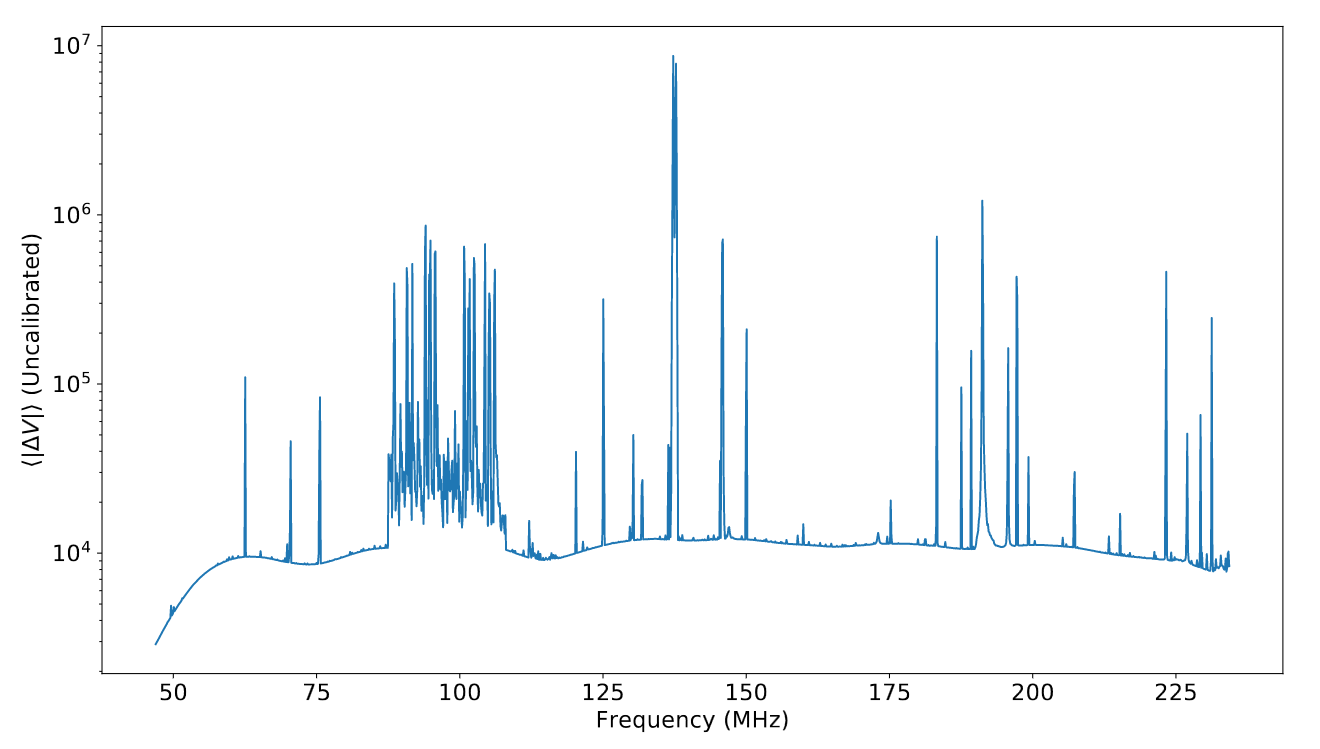
\includegraphics[width=0.9\textwidth]{rfi_example.png}

\tiny [photo credit: HERA Collaboration]

\column{0.5\textwidth}

\includegraphics[width=0.8\textwidth]{starlink.jpg}
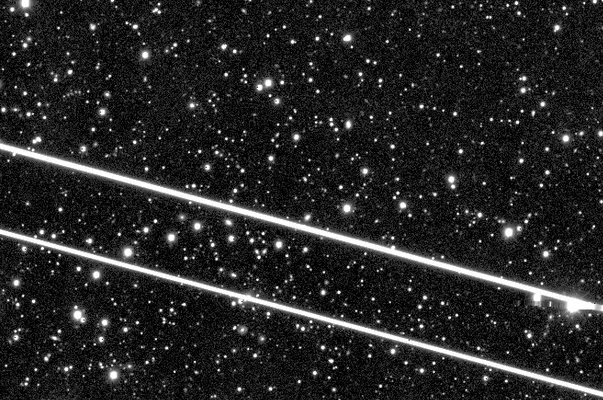
\includegraphics[width=0.8\textwidth]{starlink2.png}

\tiny [photo credit: Elon Musk?]
\end{columns}
\end{frame}


\begin{frame}{Why take a Bayesian approach?}
  \begin{block}{Many effective algorithms already exist\dots}
    \begin{itemize}
    \item Cumulative sum~\cite{baan2004radio}
    \item Single value decomposition~\cite{offringa2012morphological}.
    \item Convolutional neural nets~\cite{sun2022robust}.
    \end{itemize}
  \end{block}
  \begin{block}{Our approach}
    \begin{itemize}
    \item Can be used as part of a single step fitting process within Bayesian pipelines.
    \item Flagging and management performed simultaneously. 
    \end{itemize}
  \end{block}
\end{frame}

\begin{frame}{Bayes Theorem}
  \begin{align}
    \text{likelihood} \times \text{prior} &= \text{posterior} \times \text{evidence} \\
    P(\mathcal{D}|\theta) \times P(\theta) &= P(\theta|\mathcal{D}) \times P(\mathcal{D}), \\
    \mathcal{L} \times \pi &= \mathcal{P} \times \mathcal{Z},
\end{align}  
\end{frame}

\begin{frame}{RFI correcting likelihood}
a) Generate new likelihood capable of modeling probability data point is corrupted.
    \begin{equation}
    P(\mathcal{D}_i|\theta) = \begin{cases}
        \mathcal{L}_i(\theta) &: \text{uncorrupted}\\
        \Delta^{-1}[ 0<\mathcal{D}_i<\Delta] &: \text{corrupted},\\
    \end{cases}
\end{equation}
\end{frame}

\begin{frame}{RFI correcting likelihood}
b) Incorporate prediction of a datum containing RFI into Boolean mask $\epsilon$.
\begin{equation}
    P(\mathcal{D}|\theta, \varepsilon) = \prod_{i} \mathcal{L}_{i}^{\varepsilon_{i}} \Delta^{\varepsilon_i-1}
    \label{eq:li2}
\end{equation}
\end{frame}

\begin{frame}{RFI correcting likelihood}
c) Ascribe Bernoulli prior $P(\varepsilon_i)$ to $P(\mathcal{D} | \theta)$
\begin{equation}
        P(\varepsilon_i) = p_i^{(1-\varepsilon_i)}(1-p_i)^{\varepsilon_i}.\label{eq:pei}
        \end{equation}
\end{frame}

\begin{frame}{RFI correcting likelihood}
c) Marginalise over epsilon.
\begin{equation}
P(\mathcal{D} | \theta) =\sum_{\varepsilon \in \{ 0, 1 \} ^N}P(\mathcal{D},\varepsilon|\theta)
\end{equation}
\end{frame}

\begin{frame}{RFI correcting likelihood}
d) Assume that the correct (maximum) mask will generate a likelihood that is orders of magnitude `more likely' than all other masks. 
\begin{equation}
 P(\mathcal{D}|\theta, \varepsilon^{\mathrm{max}}) \gg P(\mathcal{D}|\theta,\varepsilon^{2})\label{eq:nlo},
\end{equation}
\begin{equation}
    P(\mathcal{D}|\theta) \approx P(\mathcal{D},\varepsilon^{\mathrm{max}}|\theta).\label{eq:approx}
\end{equation}

\end{frame}

\begin{frame}{RFI correcting likelihood}
e) Taking logs, the loglikelihood is
\begin{equation}
    \begin{aligned}
    \log{P(\mathcal{D}|\theta)} &= \sum_{i}[{\log{\mathcal{L}_i}+\log({1-p_i})]\varepsilon^{\mathrm{max}}_i + [\log{p}_i - \log{\Delta}](1 - \varepsilon^\mathrm{max}_i})\label{eq:loglikelihood},
    \end{aligned}
\end{equation}
\end{frame}

\begin{frame}
\begin{equation}
    \log{P(\mathcal{D}|\theta)} =  
    \begin{cases}
        \log \mathcal{L}_i + \log (1-p_i), &
    \begin{aligned}
        &[\log{\mathcal{L}_i} + \log({1-p_i}) \\
        &> \log p_i - \log \Delta]
    \end{aligned}\\ 
        \log p_i - \log \Delta, & \text{otherwise}.
    \end{cases}
    \label{eqn:loglcompute}
\end{equation}.
\begin{figure}
	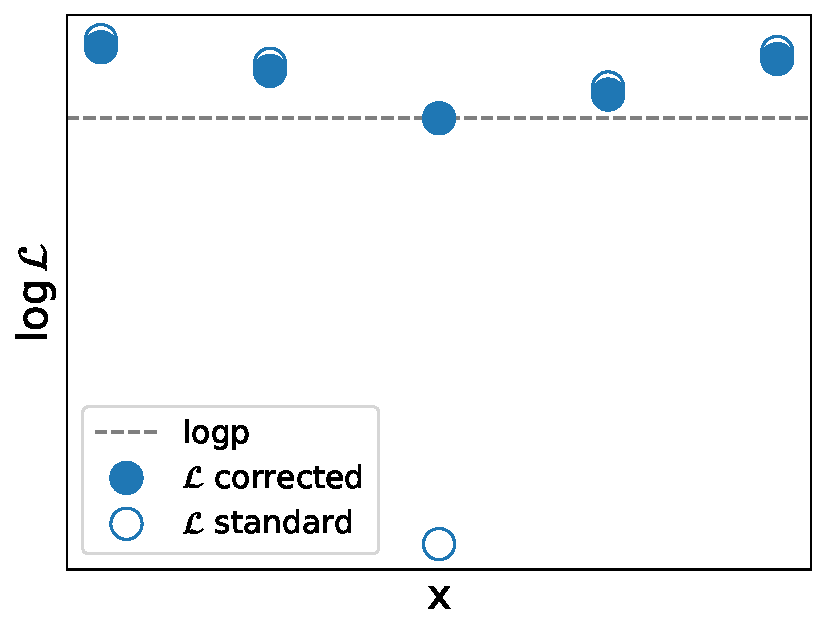
\includegraphics[width=0.7\textwidth]{theory_sketch.pdf}
\end{figure}
\end{frame}

\begin{frame}{Testing on a simple toy model}
\begin{columns}
\column{0.5\textwidth}
Using numerical sampling techniques to make predictions with $\mathcal{L}$.
\begin{itemize}
\item `Belief' in classification incorporated into model.
\item Individual datum are not excised.
\item The masks `opacity' changes based confidence of classification.
\end{itemize}
\column{0.5\textwidth}
\begin{figure}
	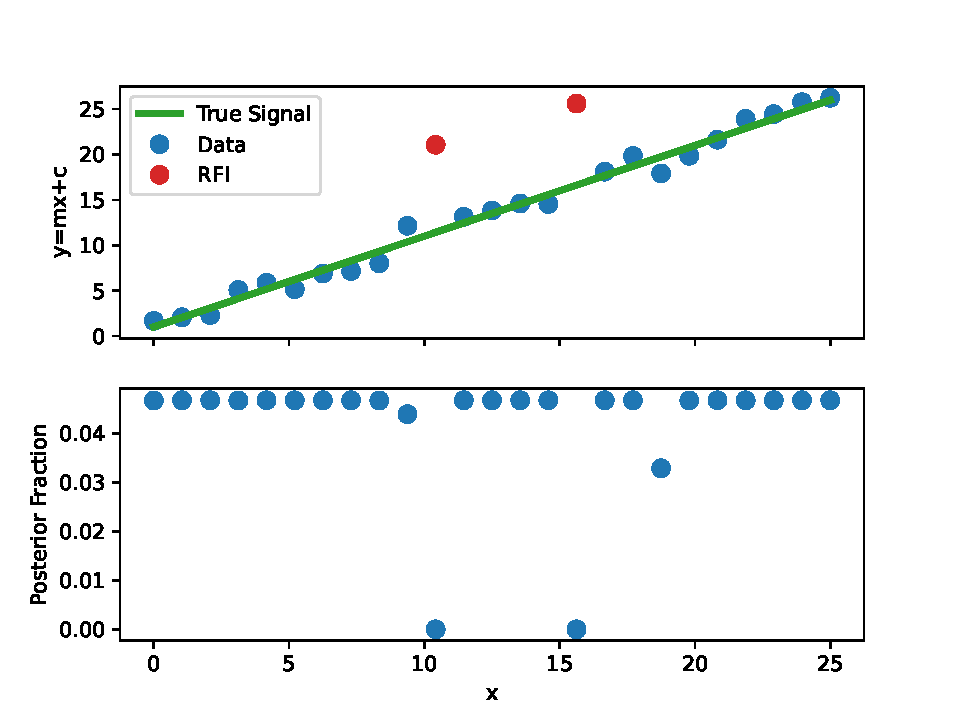
\includegraphics[width=\textwidth]{test.pdf}
\end{figure}
\end{columns}
\end{frame}

\begin{frame}{Posterior plots (basic toy model)}
\begin{figure}
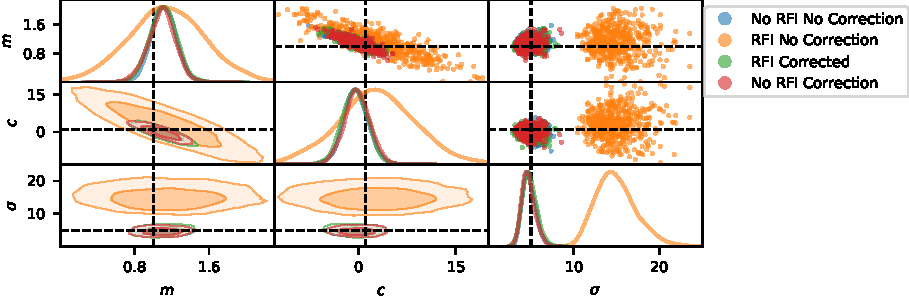
\includegraphics[width=1\textwidth]{toy9pane.pdf}
\end{figure}
\end{frame}

\begin{frame}{Testing on a simple toy model}
\begin{figure}
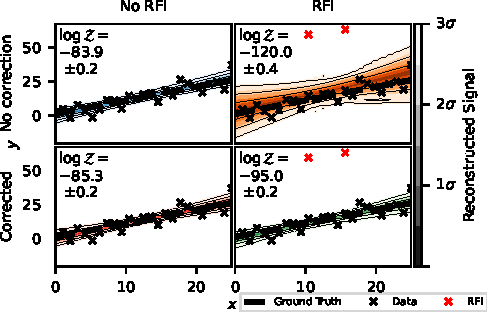
\includegraphics[width=0.75\textwidth]{4pane_toy_sidebar.pdf}
\end{figure}
\end{frame}

\begin{frame}{Probability thresholding condition $p$}
    \begin{equation}
    \begin{aligned}
    \log{P(\mathcal{D}|\theta)} &= \sum_{i}[{\log{\mathcal{L}_i}+\log({1-p_i})]\varepsilon^{\mathrm{max}} + [\log{p}_i - \log{\Delta}](1 - \varepsilon^\mathrm{max}_i})\label{eq:loglikelihood},
    \end{aligned}
    \end{equation}
\centering \animategraphics[autoplay, loop, width=11cm]{2}{gif_anest/comb_}{1}{9}
\end{frame}

\begin{frame}{Selection Strategy for $p$}
\begin{columns}
\column{0.5\textwidth}
    \begin{itemize} 
    \item `Select $p$ such that the Bayesian Evidence $\mathcal{Z}$ is maximised'
    \end{itemize}
\column{0.5\textwidth}
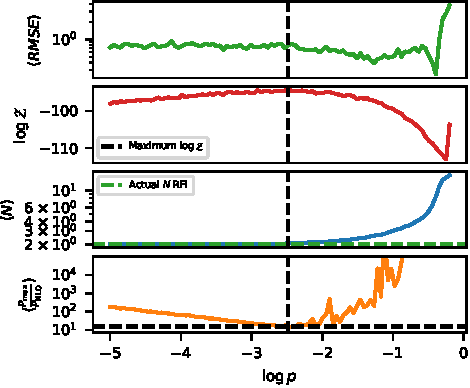
\includegraphics[width=1\textwidth]{4panevert.pdf}
\end{columns}
\end{frame}

\begin{frame}{Use case: Global 21cm Cosmology}
\centering
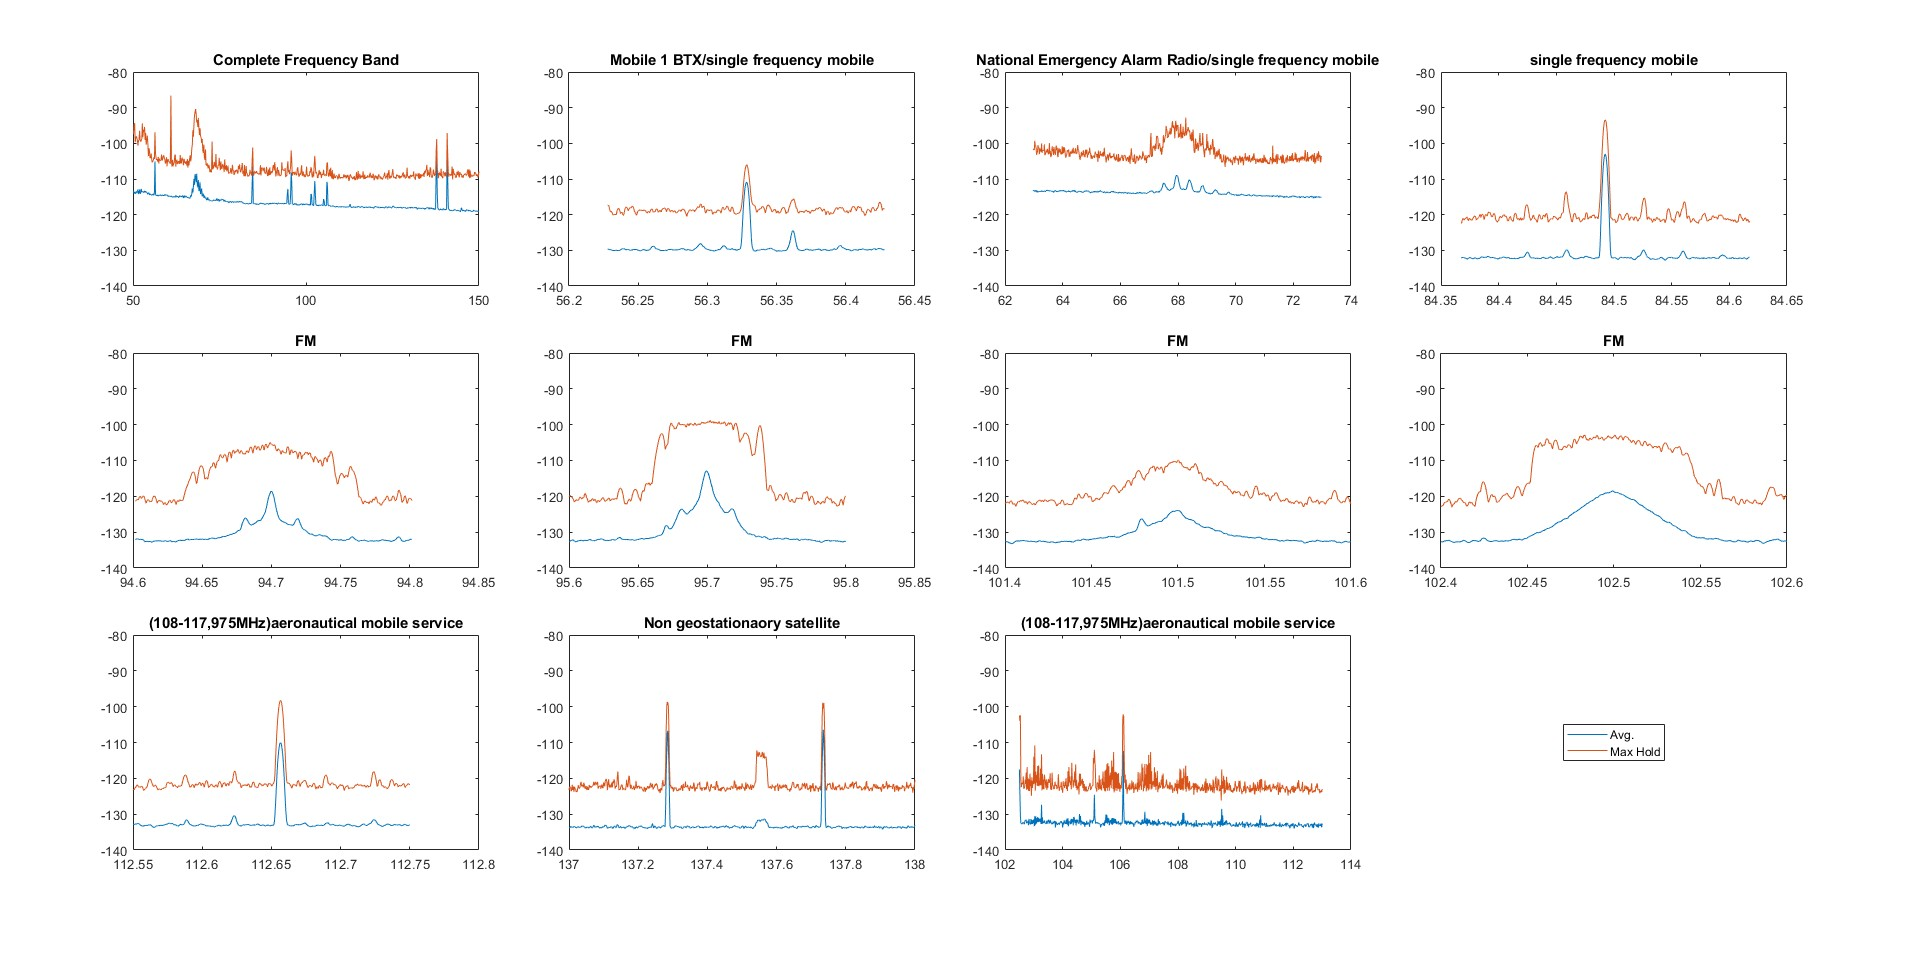
\includegraphics[width=1\textwidth]{Site Measurements March.jpg}
\end{frame}

\begin{frame}{Use case: Global 21cm Cosmology}
\centering
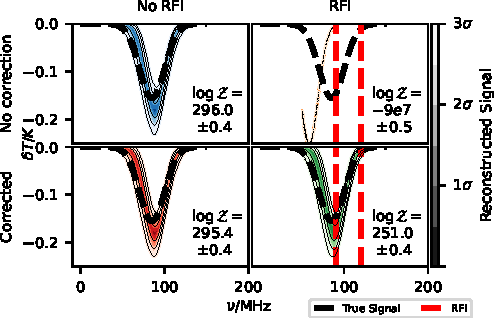
\includegraphics[width=0.8\textwidth]{4pane_reach_sidebar.pdf}
\end{frame}

\begin{frame}{General Bayesian anomaly detection?}
  
\begin{columns}
\column{0.5\textwidth}
\centering
    \begin{itemize}
    \item Can we use this to detect as well as mitigate?
    \item Extension beyond just RFI? (see Dominic's talk!)
    \item Anomalies with more complex structure?
\end{itemize}
\column{0.5\textwidth}
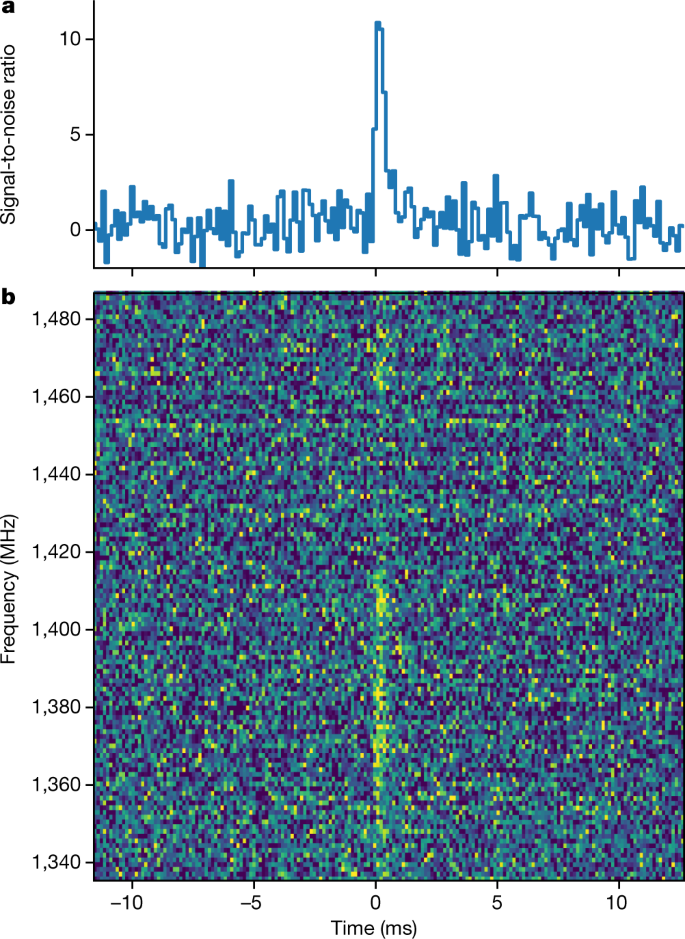
\includegraphics[width=0.8\textwidth]{frb.png}
\end{columns}
\end{frame}


\begin{frame}{Implement with 2 lines of code}
\begin{columns}
  \column{0.5\textwidth}
  
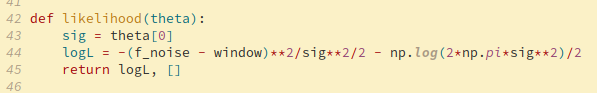
\includegraphics[width=1\textwidth]{logl1.png}
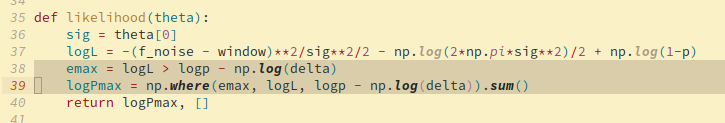
\includegraphics[width=1\textwidth]{logl2.png}

\column{0.5\textwidth}

Tutorial: https://github.com/samleeney
\end{columns}
\end{frame}


\begin{frame}{Conclusions}
So far \dots
\begin{itemize}
    \item These work serves as a proof of concept that RFI can be mitigated in a truly Bayesian sense.
    \item RFI can be mitigated as part of a single step fitting process, alongside the Bayesian Evidence and parameter estimations.
    \item Effective on a toy model and on simulated data for a global 21cm experiment.
\end{itemize}
Future Works?
\begin{itemize}
    \item Test on real data.
    \item Develop for time integrated data (see Dominic's talk!).
    \item Examine in case where data bins may be correlated.
    \item Benchmark.
\end{itemize}

\end{frame}

\begin{frame}[t]{References}
\bibliographystyle{apalike}
\bibliography{ref.bib} % if your bibtex file is called example.bib
\end{frame}




\end{document}